%\documentclass[draft,grl]{AGUTeX}
\documentclass[twocolumn,grl]{AGUTeX}
\usepackage{mathptmx}
% \usepackage{lineno}
% \linenumbers*[1]

%  To add line numbers to lines with equations:
%  \begin{linenomath*}
%  \begin{equation}
%  \end{equation}
%  \end{linenomath*}

%  Uncomment the following command to include .eps files
%  (comment out this line for draft format):
%\usepackage[dvips]{graphicx}
\usepackage[pdftex]{graphicx}
%\setkeys{Gin}{draft=false}

\authorrunninghead{STYRON AND HETLAND}
\titlerunninghead{LANF EARTHQUAKE LIKELIHOOD}

\authoraddr{Corresponding author: Richard H. Styron,
Department of Earth and Environmental Sciences, University of
Michigan, 2534 CC Little Bldg., 1100 N. University Ave., 
Ann Arbor, MI 48104, USA (richard.h.styron@gmail.com)}

\begin{document}
\title{Likelihood of observing an earthquake on a continental 
	   low-angle normal fault}

\authors{Richard H. Styron \altaffilmark{1}
and Eric A. Hetland \altaffilmark{1}}

\altaffiltext{1}{Department of Earth and Environmental Sciences, University of
Michigan, Ann Arbor, Michigan, USA.}

\begin{abstract}
Low-angle normal faults are well-described in the rock record and may serve an
important role in crustal extension.  However, a significant earthquake on
a continental low-angle normal fault has not been observed, and such slip is
often interpreted to be in conflict with standard rock mechanical theory. The
lack of observed earthquakes with focal mechanisms clearly indicating low-angle
normal slip may be an indication that they are not seismically active, or it
may be due to the fact that these earthquakes are infrequent compared to the
length of focal mechanism catalogs. To address this, we create a compilation of all
potentially active continental low-angle normal faults and calculate the
likelihood of observing a significant earthquake on them over time windows from
1 to 100 years. We find 20 candidate faults in extensional zones worldwide.  We
find that the probability of observing a significant low-angle normal fault
earthquake is dependent on several factors including the frequency-magnitude
distribution, but for either a characteristic or Gutenberg-Richter distribution
we calculate a probability of about 0.5 that an earthquake greater than $M6.5$ (and
therefore likely to have a known fault scarp and dip angle) will be observed on
any low-angle normal fault in a time window of 35 years, which is the length of
the Global CMT catalog. We then use Bayes' rule to illustrate how the absence
of observed significant low-angle normal fault seismicity over the catalog
period moderately decreases the likelihood that the structures generate
large earthquakes, but does not reduce the likelihood to zero.


\end{abstract}

\begin{article}

\section{Introduction}
Low-angle normal faults (LANFs), with dips less than 30$^\circ$, are well
described in the geologic record. They are thought to play an important role in
accommodating large-magnitude continental extension \citep{howard1987crustal}
and crustal thinning \citep{lister1986detachment}, and their recognition has
been a major development in continental tectonics
\citep{wernicke2009detachment}. However, despite widespread field observations
of inactive LANFs and their central role in extensional tectonic theory, they
remain enigmatic and contentious structures, and it is not clear if they are
seismically active at low dip angles in the upper crust. This is for two
reasons: because brittle faulting on LANFs is in apparent conflict with
standard Andersonian rock mechanical theory as typically applied to the upper
crust \citep{axen2004lanfmech}, and because observations of active faulting on
LANFs are sparse and at times ambiguous \citep{wernicke1995seis}.
A considerable amount of research has been performed to address the former
concern, reconciling LANF slip with rock mechanics \citep [e.g.,]
[]{axenbartley1997, collettini2011lanfmech}.  The latter issue is highlighted
by studies that have searched the focal mechanism catalogs and found no normal
faulting earthquakes with focal mechanisms and surface ruptures clearly
indicating slip on planes $\le30^\circ$ \citep{jackson1987,
collettinisibson2001}, which is taken as conclusive evidence that LANFs are
inactive or aseismic.  However, the lack of observed seismic slip on
continental LANFs may be simply be because they are rare structures with long
recurrence intervals, so earthquakes on them are very infrequent. Without
knowing the likelihood of observing a LANF rupture in a time window of a few
decades, it is not clear if an empty search result is strong evidence against
LANF seismicity. If this likelihood is known, though, Bayesian probability
theory provides a framework for quantifying how the negative search results
impact the probability that LANFs are seismogenic.

In this work, we estimate the maximum likelihood of a significant LANF event
occurring in time windows from 1 to 100 years, and then we interpret the lack
of observed LANF seismicity in a quantified, probabilistic context using
Bayesian methods. We estimate the maximum observation likelihood by treating
all potentially active LANFs described in the literature as seismically active
at their surface dip angles throughout the upper crust. Under these
assumptions, we create synthetic earthquake catalogs with both
Gutenberg-Richter and `characteristic' frequency--magnitude distributions,
using each fault's geometry and slip rate.  We then calculate the probability
of observing earthquakes on at least one LANF over different observation
periods. Then, we use Bayes' rule to incorporate the negative catalog search
results and the observance likelihood to show how the negative results reduce
the probability that LANFs are seismically active, but do not bring the final
probability to zero.


\subsection{LANF Slip, Mohr-Coulomb Failure Theory, and Earthquakes}

Areas of the crust undergoing active extension are generally assumed to have
a subvertical maximum compressive stress.  Mohr-Coulomb theory, as applied to
the crust, predicts that a fault with a typical coefficient of friction for
rocks (0.6--0.8) should lock up if it is oriented at an angle greater than
60$^\circ$ to the maximum compressive stress  ({\it i.e.}, fault dips less than
30$^\circ$), and new, optimally oriented faults should form \citep{sibson1985}.
Therefore, for normal faults with dips less than 30$^\circ$, either much lower
fault friction or elevated pore fluid pressure is required for fault slip.

Evidence for seismic slip on LANFs is sparse.  This is partly due to the
ambiguity of the rupture plane in earthquake focal mechanisms, and thus a focal
mechanism with a low angle nodal plane will also have a high angle nodal plane.
Without ancillary information indicating which nodal plane corresponds to the
slip surface, searches of earthquake catalogs cannot yield unique results as to
whether they contain LANF events. Several collections of normal fault
earthquakes with known surface breaks \citep{jackson1987,
collettinisibson2001}, thereby resolving dip ambiguity, contain no low-angle
events, although we note the total number of events in these collections are
small ($\le$ 25 events).  Some candidate LANF events exist, but they are
undersea \citep[e.g.,][]{abers2001} or difficult to verify \citep[e.g.,]
[]{doser1987ancash}.


\section{Potentially Active LANFs}

Over the past decade or so, many field studies have found evidence for LANF
activity in orogens throughout the world. These studies typically find arrays
of Quaternary normal fault scarps on the fault traces and/or in the hanging
walls of mapped or inferred low-angle detachment faults \citep [e.g.,]
[]{axen1999baja}. Some studies also have bedrock thermochronology data from the
exhumed detachment footwalls that are suggestive of ongoing rapid exhumation
\citep [e.g.,][]{sundell2013lunggar}, although this data does not preclude
a recent cessation of faulting. In some cases, additional evidence for LANF
activity comes from geophysical data such as GPS geodesy \citep [e.g.,]
[]{hreinsdottir2009altotib} and seismic waves \citep
[e.g.,][]{doser1987ancash}.

\begin{figure*}%[th]
\noindent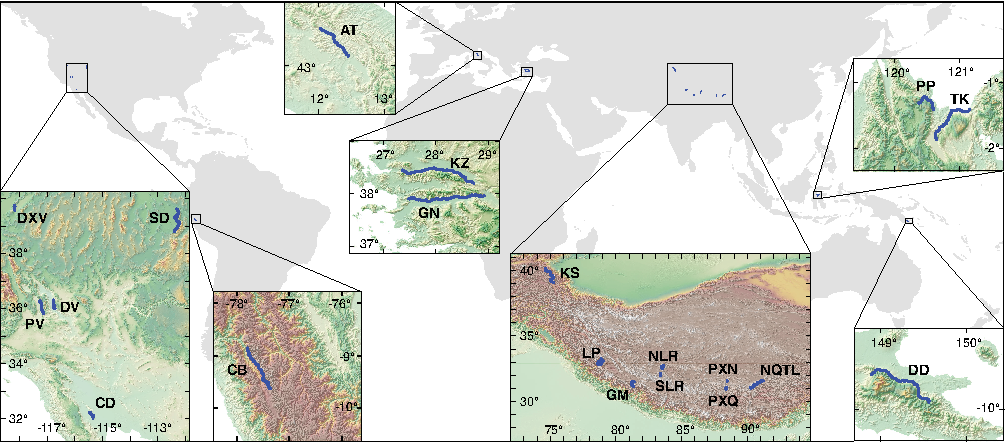
\includegraphics[width=40pc]{./figures/active_lanfs_map_insets.pdf}
\caption{Map of known, potentially active continental LANFs (blue lines), with
insets showing the physiographic context of the faults.  DXV=Dixie Valley
fault.  PV=Panamint Valley fault.  DV=Death Valley fault.  CD=Ca\~nada David
detachment.  SD=Sevier Desert detachment.  CB=Cordillera Blanca detachment.  
AT=Alto-Tiberina fault.  KZ=Kuzey detachment.  GN=Guney detachment.  
KS=Kongur Shan fault.  LP=Leo Pargil detachment.  GM=Gurla Mandhata 
detachment. NLR=North Lunggar detachment.  SLR=South Lunggar detachment.  
PXN=Pum Qu--Xainza north fault.  PXQ=Pum Qu--Xainza Qingdu fault. 
NQTL=Nyainqentanglha detachment.  PP=Pompangeo detachment.  
TK=Tokorondo detachment.  DD=Dayman Dome.}
\label{fig:lanf_map}
\end{figure*}

We have compiled all potentially active LANFs with known subareal fault traces
from a thorough review of the literature, finding twenty total
(Figure~\ref{fig:lanf_map}).  We have then mapped the approximate fault traces
into a GIS file (available at https://github.com/cossatot/LANF\_gis), with
metadata such as slip rate and source. Though the fault traces of many LANFs
considered here are obscured by vegetation, others display large fault scarps
in Quaternary sediments, particularly those in Tibet
\citep[e.g.,][]{styron2013slr, kapp2005nqtl} and the western US
\citep[e.g.,][]{axen1999baja, hayman2003dv}, which are commonly interpreted as
evidence for past seismic slip.  About half are in Tibet, consistent with
hypotheses that LANFs and metamorphic core complexes form in areas of hot,
thick crust \citep [e.g.,][]{buck1991mcc}.  The rest are distributed through
other areas of active continental extension: the North American Basin and
Range, the Malay Archipelago, western Turkey, Italy, and Peru. 

Several of the most-commonly cited candidates for seismically active LANFs were
not included because they do not have a clearly-defined, mappable fault trace,
which is necessary for our earthquake likelihood calculations.  These include
the 1995 Aigion, Greece earthquake fault \citep{bernard1997} and other
potential LANFs underneath the Gulf of Corinth, and the 1952 Ancash, Peru
earthquake fault \citep{doser1987ancash}. Furthermore, though submarine core
complexes with superficially low-angle detachments are well-described in the
literature and some of these structures may have produced recent earthquakes
\citep{abers2001}, we do not include these in our calculations for several
reasons: because mid-ocean ridges have not been structurally mapped with the
completeness or resolution of subareal extensional provinces, it is not
currently possible to come up with a reasonably complete inventory of ocean
LANFs; without high-resolution structural mapping and geodesy of oceanic LANFs,
it is not possible to determine which structures in a mid-ocean ridge segment
are currently active (seismically or not), and it is difficult to confidently
associate particular earthquakes with a specific fault, given the high spatial
density of normal faults at mid-ocean ridges.


\section{Likelihood of observing a LANF event}
\subsection{Earthquake Likelihood on Individual LANFs}
To estimate the likelihood of observing a significant earthquake on an
individual LANF over some contiguous time window of length $t$ (in years), we
perform a Monte Carlo simulation in which we create 4000 synthetic time series
of earthquakes, with unique values for fault geometry and slip rate for each
time series. Then, for each time series we calculate the fraction of unique
time windows of length $t$ in which an earthquake as large or larger than
a given magnitude occurs.  We take this value as the probability of observing
an earthquake greater than or equal to moment magnitude \emph{M} over time
period $t$, which we will refer to in general as $P(M,t)$.  All calculations
are performed with Python, with usage of the Numpy \citep{oliphant2007numpy},
IPython \citep{perez2007ipython}, Pandas, and Joblib Parallel
\citep{varoquaux_joblib} packages.  All code and data for this project is
available at https://github.com/cossatot/lanf\_earthquake\_likelihood/.

The geometry for each fault is estimated based on the length of the fault
trace, the dip of the fault, and the estimated fault locking depth in the area.
The fault is treated as planar for simplicity of calculations, even though the
exposed footwalls of many detachment faults are nonplanar.  We determine the
fault length by measuring the approximate length of the mapped fault trace
perpendicular to the assumed extension direction; for faults that change dip
significantly along strike, we only consider the low-angle segments of the
fault.  Values for the dip are taken from the literature in most cases, and
measurements of the dip of footwall triangular facets (interpreted as the
exhumed fault plane) from SRTM data otherwise. In all cases, ranges of fault
geometries are considered, encompassing the degree to which the values are
known. The fault locking depth is assumed to be 10 km in the absence of other
evidence (such as a geodetic study, \citep[e.g.,][]{hreinsdottir2009altotib}).

Slip rates of the 20 LANFs are gathered from the literature if possible, or
given broad ranges if not (e.g., 1--10 mm yr$^{-1}$).  In the Monte Carlo
simulation, samples for slip rate and dip are drawn from uniform distributions
defined by the maximum and minimum values.  Based on field observations, some
faults have dip ranges that go above 30$^\circ$, although for these faults dip
values are sampled from the minimum to 30$^\circ$, as here we only consider
slip on faults shallower than 30$^\circ$. The resulting probabilities on these
faults are then multiplied by the fraction of the dip range that is
$\le30^\circ$.

\begin{figure}[b]
\noindent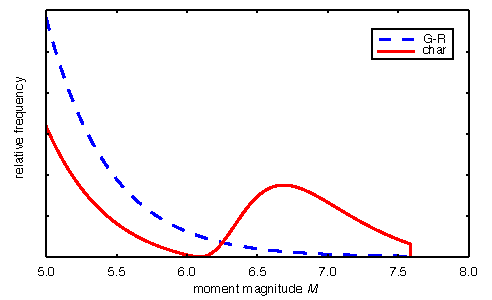
\includegraphics[width=20pc]{./figures/F-Ms.pdf}
\caption{Gutenberg-Richter and characteristic frequency-magnitude 
 		 distributions for the South Lunggar detachment}
\label{fig:fms}
\end{figure}

Each synthetic earthquake sequence is generated by randomly sampling either
50,000 events from a tapered Gutenberg-Richter (GR) distribution with corner
magnitude $M_c = 7.64$ and $\beta = 0.65$ (from values estimated by
\citet{birdkagan2004f_m} for continental rifts), or a 25,000 events from
`characteristic' distribution. It is not certain which distribution more
appropriately describes seismicity on a single LANF, though studies of many
individual fault rupture histories suggests that the characteristic
distribution is more accurate \citep{hecker2013eqdist}.  The smaller number of
samples from the characteristic distribution is due to the increased
computation time associated with a higher proportion of large events, leading
to much longer time series for a given number of events.  The samples are taken
from an interval $M = [5.0, \, M_{max}]$, where $M_{max}$ is the moment
magnitude associated with 15 m of slip over the given fault plane.  We use the
standard relations between fault slip, $D$, and moment magnitude, $M$, given by

\begin{equation}
 M_o = \mu L z D \,/ \, \sin \delta 
 \end{equation}

and

\begin{equation}
M = 2/3 \; \log_{10} (M_o) - 6
\end{equation}
where $L$ is the fault length, $z$ is the seismogenic thickness, $\delta$ is
the fault dip, $\mu = 30$ GPa is the shear modulus, and $M_o$ is the seismic
moment in N m \citep{kagan2003pepi}.  The characteristic distribution has
a large-magnitude mode corresponding to $D$ = 1.5 m on the fault, a typical
slip distance for normal fault events
\citep[e.g.][]{wesnousky2008displacement}.  The distributions are shown in
Figure~\ref{fig:fms}.

These calculations rely on two important assumptions that warrant some
discussion.  The first is that each earthquake ruptures the entire fault patch
uniformly.  Though this is unlikely fault behavior, the long-term statistical
distribution of earthquake recurrence is insensitive to assumptions about slip
distribution in individual events as long as earthquakes are unclustered in
time (the second assumption discussed below).  Specifically, if $n$ different,
equal fault patches rupture independently, each requires $n$ times the
interseismic strain accumulation time to rupture with an earthquake of
magnitude $M$ compared to the accumulation time for a single fault rupturing
uniformly with much lower coseismic slip in each earthquake. Thus, magnitude
$M$ events would happen with the same long-term frequency.  The next assumption
is that earthquakes are ordered randomly and separated by the time necessary
for sufficient strain to accumulate for each earthquake to occur.  This means
that foreshock and aftershock sequences and other types of event clustering are
not taken into account.  However, the modal inter-event times for earthquakes
$\ge M \,6$ or so are greater than a hundred years for most LANFs, so the
ordering of events does not impact the results, as this is longer than our
maximum observation window.  Furthermore, any clustering resulting in event
spacing less than the observation window would decrease $P(M,t)$, and here we
choose to calculate the maximum $P(M,t)$ using the simplest assumptions, rather
that choose the model assumptions such that the calculated probabilities are
the minimum.

The results for faults with a GR frequency-magnitude distribution indicate that
it is unlikely that any individual fault would have an earthquake greater than
$M \, 5$ in any modeled observation time up to 100 years.
As an example, the results for the Panamint Valley fault are shown in
Figure~\ref{fig:pv}a; this fault has the highest $P(M,t)$ of any of the
well-studied LANFs.  The probability of observing a $\ge M \, 6.0$ event on the
Panamint Valley fault is about 0.5 for $t$ = 100 years, and about 0.15 for $t$
= 35 years, which is the length of the Global CMT catalog. As expected given
the GR distribution, the $P(M,t)$ is much higher for smaller, more frequent
events than for larger events.  

The results for faults with a characteristic frequency-magnitude distribution
yield much lower $P(M,t)$ for small to moderate events, but $P(M,t)$ is higher
for large events(Figure~\ref{fig:pv}b,d); this is because the earthquake
sequences are dominated by large, infrequent events, so the inter-event times
for moderate events are several times greater. For the Panamint Valley fault,
$P(M\ge5,t=35)$ is about 0.07 (versus 0.25 for the GR distribution), but
$P(M\ge 7, t=35)$ is around 0.025 (versus essentially zero for the GR
distribution).  As the characteristic distribution likely better represents
earthquakes on an individual large fault, these results suggest that is very
unlikely that we would expect to capture any significant seismicity on an
single LANF in the focal mechanism catalogs. A similar conclusion was found by
\citet{wernicke1995seis} based on a simple calculation, assuming perfectly
repeating large earthquakes on an idealized fault. 
 
\begin{figure}[th]
	\noindent\includegraphics[width=20pc]{./figures/pv_probs.pdf}
	\caption{\textbf{a:} Probabilities of observing an earthquake greater than
	or equal to a given moment magnitude \emph{M} over a given observation
	window on the Panamint Valley fault, for the Gutenberg-Richter
	distribution.  \textbf{b:} Probabilities of observing an earthquake greater
	than or equal to a given moment magnitude \emph{M} over a given observation
	window on the Panamint Valley fault, for the characteristic distribution.
	Note the change in the scale of the y axis.  \textbf{c:} Cross-section
	through \textbf{a} at $t$ = 35 years, showing the distributions of $P(M)$.
	\textbf{d:} Cross-section through \textbf{b} at $t$ = 35 years, showing the
distributions of $P(M)$.} \label{fig:pv} \end{figure}

\subsection{Earthquake Likelihood on All LANFs}
To calculate the probability of observing at least one earthquake on \emph{any}
of these LANFs during a given time period, we first assume that seismicity on
each fault is independent and uncorrelated with seismicity on all other faults.
This assumption is likely true for most faults, but may not be true for the few
proximal faults, though it is unclear how these faults may interact such that
an appropriate joint probability may be calculated.  We determine the
probability for each time window and minimum magnitude with the equation
\begin{equation}
P_{AT \, or \, LP\, or\, \ldots \, or \, DV} = 1 - (Q_{AT} \cdot Q_{LP} \cdot \ldots \, \cdot Q_{DV})
\label{ProbUnion}
\end{equation}
where $P_{AT}$ is the probability of observing an earthquake on a single LANF
(e.g., the Alto-Tiberina fault), and $Q_{AT} = 1 - P_{AT}$. Equation
(\ref{ProbUnion}) is the union of probabilities for non-mutually exclusive
random events.

The results of this calculation are shown in Figure~\ref{fig:all_probs} a and b.
For the Gutenberg-Richter distribution, the likelihood of observing a LANF
earthquake on \emph{any} fault over a given observation period is quite high.
For example, $P(M,t)$ for $M \, \ge 6$ and $t$ = 35 years is about 0.85, and
for the smaller events is quite close to 1.  This high likelihood suggests that
given the model assumptions, we should expect to find such an earthquake in the
focal mechanism catalogs, though because many $M6$ events are not
surface-breaking \citep{hecker2013eqdist}, it might be difficult to
unambiguously determine whether the high- or low-angle nodal plane slipped.
%This ambiguity in fault plane would make it difficult to determine if the
%focal mechanism corresponded to a LANF earthquake or a high angle normal fault
%earthquake. 
For $M \, \ge 6.5$, the probability of observing a LANF earthquake is about
0.5, and the nodal plane ambiguity should be much less ({\it e.g.}, due to
surface scarps or directivity effects).  The results for the characteristic
distribution are lower than the results for the GR distribution for smaller
events and higher for larger events, similar to the patterns seen in results
for individual faults. $P(M\ge5.5,t)$ through $P(M\ge6.5)$ are all close, about
0.4--0.5.


\begin{figure*}%[t!]
\noindent\includegraphics[width=40pc]{./figures/all_probs_2x2.pdf}

\caption{\textbf{a:} Probabilities of observing an earthquake greater than or
equal to a given moment magnitude \emph{M} over a given observation window on
any LANF, given a Gutenberg-Richter distribution.  \textbf{b:} Probabilities of
observing an earthquake greater than or equal to a given moment magnitude
\emph{M} over a given observation window on any LANF, given a characteristic
distribution.  \textbf{c:} Cross-section through \textbf{a} at $t$ = 35 years
showing probability distributions.  \textbf{d:} Cross-section through
\textbf{b} at $t$ = 35 years showing probability distributions.}

\label{fig:all_probs}
\end{figure*}

\subsection{Bayesian adjustments of LANF earthquake likelihood}

Because the earthquake focal mechanism catalog is much shorter than the repeat
time for moderate to large earthquakes on typical normal faults with mm
yr$^{-1}$ slip rates, catalog searches yielding no results for a particular
class of events cannot be definitive evidence that they do not occur, but
nonetheless do provide some evidence against their existence. Through Bayes'
rule, we can use the likelihood of observing an event (\emph{i.e.}, our
calculated $P(M,t)$) to quantitatively interpret the null result in the catalog
searches. This interpretation does not produce a single probability for LANF
seismicity, but instead gives an adjusted, posterior likelihood for a given
prior likelihood that may be based on any ancillary evidence.  In this study,
we do not set a specific prior for LANF seismicity; different priors may result
from different evidence or assumptions, and are not likely to be constant
through time or among all researchers.  Instead, we calculate the posteriors
over the full range of prior probabilities [0,1]. Here $P(A)$ represents the
prior probability for LANF seismic activity, and $P(O)$ is a positive test
result (observation of a LANF earthquake in a catalog search).  The symbol
`$\sim$' indicates \emph{not}, so $P(\sim A)$ is the probability of LANF
inactivity, equal to $ 1 - P(A)$.  The results of this study gives the us the
probability of observing or not observing a LANF event given LANF seismic
activity, $P(O|A)$ and $P(\sim O | A) = 1 - P(O|A)$, respectively. $P(O | \sim
A)$ is the probability of observing a `false positive', the incorrect
identification of a LANF event.  The posterior $P(A |\sim O)$ is the likelihood
of LANF activity given that no LANF events have been observed.  This result is
obtained through a form of Bayes' rule for binary outcomes

\begin{equation}
P(A | \sim O) = \frac{P(\sim O|A) P(A)}
{P(\sim O|A)P(A) + P(\sim O|\sim A)P(\sim A)}
\label{BayesRule}
\end{equation}

Figure~\ref{fig:posteriors} shows $P(A|\sim O)$ for $P(A) = [0,1]$,
using values for $P(O|A)$ of 0.1, 0.5, and 0.8, and a likelihood of false positives $P(O|\sim A)= 0.01$. It is evident in these results that the likelihood of LANF seismicity decreases appreciably given a moderate $P(O|A)$, and decreases significantly given a higher $P(O|A)$, but the values do not decrease to zero.


\section{Discussion and Conclusions}

Our compilation of all known potentially active LANFs shows that they are
fairly uncommon structures, yet they still may be found in areas currently
undergoing extension. Almost all major continental extensional regions are
represented; notably, narrow, linear continental rifts, such as the East
African and Rio Grande rifts, do not seem to contain active LANFs.  This
compilation may serve as a point of comparison for different characteristics of
active normal faults or LANF geometry, or as a reference for any further
related study of these structures.

$P(M\ge6.5, t=35)$ is about 0.5 for either frequency--magnitude distribution,
and events in this range are likely to be surface- breaking, and therefore have
unambiguous slip planes, unlike smaller events \citep{hecker2013eqdist};
therefore, this value is a good reference value for discussion.  This value is
a maximum estimate, because we assume that all LANFs in this study are
seismically active throughout the upper crust at surface dip angles.  It is
quite possible that some of these faults are not tectonically active at all. It
is also possible that some or all of these detachments may be seismically
active but at dip angles $\ge30^\circ$.  For example, the Ca\~nada David
detachment in Mexico may dip very steeply at seismogenic depths
\citep{fletcherspelz2009}.  Some of these may also be aseismic; the
Alto-Tiberina fault appears to be creeping for much of its down-dip extent
\citep{hreinsdottir2009altotib}, and the neighboring Zuccale inactive LANF has
fault gouge suggestive of creep  \citep{collettiniholdsworth2004}.

The likelihood of LANF seismicity for $P(M\ge6.5, t=35) = P(O|A) = 0.5 $ is
only somewhat decreased after no observations in the focal mechanisms catalogs;
although the magnitude of the decrease depends on the prior likelihood, the
decrease is at most $\sim 15 \%$. This means that the current catalog length is
much too short to be used as strong evidence against LANF seismicity.
$P(M\ge6.5, t=100)$ is near 0.8 for both GR and characteristic distributions;
this value more strongly reduces the likelihood of LANF seismicity, yet still
does not yield a definitive negative conclusion.  Therefore, results of studies
analyzing the dip distribution of earthquakes on continental normal faults
\citep{jackson1987, collettinisibson2001} should be interpreted as informative
but not conclusive. Furthermore, alternative mechanisms for LANF occurrence or
slip such as aseismic creep \citep [e.g.,][]{collettini2011lanfmech,
hreinsdottir2009altotib}, isostatic flexure \citep[e.g.,][]
{wernickeaxen1988rolling}, or extremely long seismic recurrence intervals
\citep{wernicke1995seis} need not be invoked to explain the lack of observed
seismicity, though these mechanisms may indeed be valid or well supported by
other observations.


\begin{figure}%[h]
%\noindent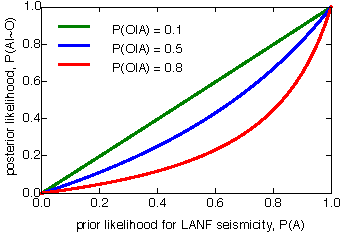
\includegraphics[width=20pc]{./figures/posteriors.pdf}
 \noindent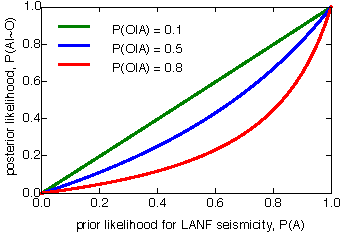
\includegraphics{./figures/posteriors.pdf}
 \caption{Prior likelihood for LANF seismicity $P(A)$ and posterior
 likelihood $P(A|\sim O)$ given no observed earthquakes.  
 $P(O|A)$ is the likelihood of observing an earthquake given activity
 on all LANFs.}
 \label{fig:posteriors}
\end{figure}

\begin{acknowledgements}
  We thank Jon Spencer for a stimulating discussion that became the impetus for
  this study.  Mike Taylor and Kurt Sundell provided valuable comments on
  a draft of the manuscript. 
 
\end{acknowledgements}

% put bib here
\begin{thebibliography}{30}
\providecommand{\natexlab}[1]{#1}
\expandafter\ifx\csname urlstyle\endcsname\relax
  \providecommand{\doi}[1]{doi:\discretionary{}{}{}#1}\else
  \providecommand{\doi}{doi:\discretionary{}{}{}\begingroup
  \urlstyle{rm}\Url}\fi

\bibitem[{\textit{Abers}(2001)}]{abers2001}
Abers, G.~A. (2001), Evidence for seismogenic normal faults at shallow dips in
  continental rifts, \textit{Geological Society, London, Special Publications},
  \textit{187}(1), 305--318.

\bibitem[{\textit{Axen}(2004)}]{axen2004lanfmech}
Axen, G.~J. (2004), Mechanics of low-angle normal faults, in \textit{Rheology
  and Deformation of the Lithosphere at Continental Margins}, edited by G.~D.
  Karner et~al., pp. 46--91, Columbia Univ. Press, New York.

\bibitem[{\textit{Axen and Bartley}(1997)}]{axenbartley1997}
Axen, G.~J., and J.~M. Bartley (1997), Field tests of rolling hinges:
  Existence, mechanical types, and implications for extensional tectonics,
  \textit{Journal of Geophysical Research}, \textit{102}(B9), 20,515--20.

\bibitem[{\textit{Axen et~al.}(1999)\textit{Axen, Fletcher, Cowgill, Murphy,
  Kapp, MacMillan, Ramos-Vel{\'a}zquez, and Aranda-G{\'o}mez}}]{axen1999baja}
Axen, G.~J., J.~M. Fletcher, E.~Cowgill, M.~Murphy, P.~Kapp, I.~MacMillan,
  E.~Ramos-Vel{\'a}zquez, and J.~Aranda-G{\'o}mez (1999), Range-front fault
  scarps of the sierra el mayor, baja california: Formed above an active
  low-angle normal fault?, \textit{Geology}, \textit{27}(3), 247--250.

\bibitem[{\textit{Bernard et~al.}(1997)\textit{Bernard, Briole, Meyer,
  Lyon-Caen, Gomez, Tiberi, Berge, Cattin, Hatzfeld, Lachet
  et~al.}}]{bernard1997}
Bernard, P., P.~Briole, B.~Meyer, H.~Lyon-Caen, J.-M. Gomez, C.~Tiberi,
  C.~Berge, R.~Cattin, D.~Hatzfeld, C.~Lachet, et~al. (1997), The ms= 6.2, june
  15, 1995 aigion earthquake (greece): evidence for low angle normal faulting
  in the corinth rift, \textit{Journal of Seismology}, \textit{1}(2), 131--150.

\bibitem[{\textit{Bird and Kagan}(2004)}]{birdkagan2004f_m}
Bird, P., and Y.~Y. Kagan (2004), Plate-tectonic analysis of shallow
  seismicity: Apparent boundary width, beta, corner magnitude, coupled
  lithosphere thickness, and coupling in seven tectonic settings,
  \textit{Bulletin of the Seismological Society of America}, \textit{94}(6),
  2380--2399.

\bibitem[{\textit{Buck}(1991)}]{buck1991mcc}
Buck, W.~R. (1991), Modes of continental lithospheric extension,
  \textit{Journal of Geophysical Research: Solid Earth (1978--2012)},
  \textit{96}(B12), 20,161--20,178.

\bibitem[{\textit{Collettini}(2011)}]{collettini2011lanfmech}
Collettini, C. (2011), The mechanical paradox of low-angle normal faults:
  Current understanding and open questions, \textit{Tectonophysics},
  \textit{510}(3), 253--268.

\bibitem[{\textit{Collettini and Holdsworth}(2004)}]{collettiniholdsworth2004}
Collettini, C., and R.~Holdsworth (2004), Fault zone weakening and character of
  slip along low-angle normal faults: insights from the {Z}uccale fault,
  {E}lba, {I}taly, \textit{Journal of the Geological Society}, \textit{161}(6),
  1039--1051.

\bibitem[{\textit{Collettini and Sibson}(2001)}]{collettinisibson2001}
Collettini, C., and R.~H. Sibson (2001), Normal faults, normal friction?,
  \textit{Geology}, \textit{29}(10), 927--930.

\bibitem[{\textit{Doser}(1987)}]{doser1987ancash}
	Doser, D.~I. (1987), The {A}ncash, {P}eru, earthquake of 1946 {N}ovember
10: Evidence for low-angle normal faulting in the high {A}ndes of northern
	{P}eru, \textit{Geophysical Journal of the Royal Astronomical Society},
	\textit{91}(1), 57--71.

\bibitem[{\textit{Fletcher and Spelz}(2009)}]{fletcherspelz2009}
Fletcher, J.~M., and R.~M. Spelz (2009), Patterns of {Q}uaternary deformation
  and rupture propagation associated with an active low-angle normal fault,
  {L}aguna {S}alada, {M}exico: Evidence of a rolling hinge?,
  \textit{Geosphere}, \textit{5}(4), 385--407.

\bibitem[{\textit{Hayman et~al.}(2003)\textit{Hayman, Knott, Cowan, Nemser, and
  Sarna-Wojcicki}}]{hayman2003dv}
Hayman, N.~W., J.~R. Knott, D.~S. Cowan, E.~Nemser, and A.~M. Sarna-Wojcicki
  (2003), Quaternary low-angle slip on detachment faults in {D}eath {V}alley,
  {C}alifornia, \textit{Geology}, \textit{31}(4), 343--346.

\bibitem[{\textit{Hecker et~al.}(2013)\textit{Hecker, Abrahamson, and
  Wooddell}}]{hecker2013eqdist}
Hecker, S., N.~Abrahamson, and K.~Wooddell (2013), Variability of displacement
  at a point: Implications for earthquake-size distribution and rupture hazard
  on faults, \textit{Bulletin of the Seismological Society of America},
  \textit{103}(2A), 651--674.

\bibitem[{\textit{Howard and John}(1987)}]{howard1987crustal}
Howard, K.~A., and B.~E. John (1987), Crustal extension along a rooted system
  of imbricate low-angle faults: {Colorado River} extensional corridor,
  {California} and {Arizona}, \textit{Geological Society, London, Special
  Publications}, \textit{28}(1), 299--311.

\bibitem[{\textit{Hreinsd{\'o}ttir and
  Bennett}(2009)}]{hreinsdottir2009altotib}
Hreinsd{\'o}ttir, S., and R.~A. Bennett (2009), Active aseismic creep on the
  alto tiberina low-angle normal fault, italy, \textit{Geology},
  \textit{37}(8), 683--686.

\bibitem[{\textit{Jackson}(1987)}]{jackson1987}
Jackson, J. (1987), Active normal faulting and crustal extension,
  \textit{Geological Society, London, Special Publications}, \textit{28}(1),
  3--17.

\bibitem[{\textit{Kagan}(2003)}]{kagan2003pepi}
Kagan, Y.~Y. (2003), Accuracy of modern global earthquake catalogs,
  \textit{Physics of the Earth and Planetary Interiors}, \textit{135}(2),
  173--209.

\bibitem[{\textit{Kapp et~al.}(2005)\textit{Kapp, Harrison, Kapp, Grove,
  Lovera, and Lin}}]{kapp2005nqtl}
Kapp, J.~L., T.~M. Harrison, P.~Kapp, M.~Grove, O.~M. Lovera, and D.~Lin
  (2005), Nyainqentanglha {S}han: a window into the tectonic, thermal, and
  geochemical evolution of the {L}hasa block, southern {T}ibet, \textit{Journal
  of Geophysical Research: Solid Earth (1978--2012)}, \textit{110}(B8).

\bibitem[{\textit{Lister et~al.}(1986)\textit{Lister, Etheridge, and
  Symonds}}]{lister1986detachment}
Lister, G., M.~Etheridge, and P.~Symonds (1986), Detachment faulting and the
  evolution of passive continental margins, \textit{Geology}, \textit{14}(3),
  246--250.

\bibitem[{\textit{Oliphant}(2007)}]{oliphant2007numpy}
Oliphant, T.~E. (2007), Python for scientific computing, \textit{Computing in
  Science \& Engineering}, \textit{9}(3), 10--20.

\bibitem[{\textit{P\'erez and Granger}(2007)}]{perez2007ipython}
P\'erez, F., and B.~E. Granger (2007), {IP}ython: a {S}ystem for {I}nteractive
  {S}cientific {C}omputing, \textit{{C}omput. {S}ci. {E}ng.}, \textit{9}(3),
  21--29.

\bibitem[{\textit{Sibson}(1985)}]{sibson1985}
Sibson, R.~H. (1985), A note on fault reactivation, \textit{Journal of
  Structural Geology}, \textit{7}(6), 751--754.

\bibitem[{\textit{Styron et~al.}(2013)\textit{Styron, Taylor, Sundell, Stockli,
  Oalmann, M{\"o}ller, McCallister, Liu, and Ding}}]{styron2013slr}
Styron, R.~H., M.~H. Taylor, K.~E. Sundell, D.~F. Stockli, J.~A. Oalmann,
  A.~M{\"o}ller, A.~T. McCallister, D.~Liu, and L.~Ding (2013), Miocene
  initiation and acceleration of extension in the {S}outh {L}unggar rift,
  western {T}ibet: Evolution of an active detachment system from structural
  mapping and ({U}-{T}h)/{H}e thermochronology, \textit{Tectonics},
  \textit{32}(4), 880--907, \doi{10.1002/tect.20053}.

\bibitem[{\textit{Sundell et~al.}(2013)\textit{Sundell, Taylor, Styron,
  Stockli, Kapp, Hager, Liu, and Ding}}]{sundell2013lunggar}
Sundell, K.~E., M.~H. Taylor, R.~H. Styron, D.~F. Stockli, P.~Kapp, C.~Hager,
D.~Liu, and L.~Ding (2013), Evidence for constriction and {P}liocene
acceleration of east-west extension in the {N}orth {L}unggar rift region of west
central {T}ibet, \textit{Tectonics}, \textit{32}(5), 1454--1479,
  \doi{10.1002/tect.20086}.

\bibitem[{\textit{Varoquaux and Grisel}(2009)}]{varoquaux_joblib}
Varoquaux, G., and O.~Grisel (2009), {J}oblib: {R}unning {P}ython function as
pipeline jobs, http://pythonhosted.org/joblib/.

\bibitem[{\textit{Wernicke}(1995)}]{wernicke1995seis}
Wernicke, B. (1995), Low-angle normal faults and seismicity: A review,
  \textit{Journal of Geophysical Research}, \textit{100}(B10), 20,159--20.

\bibitem[{\textit{Wernicke}(2009)}]{wernicke2009detachment}
Wernicke, B. (2009), The detachment era (1977--1982) and its role in
  revolutionizing continental tectonics, \textit{Geological Society, London,
  Special Publications}, \textit{321}(1), 1--8.

\bibitem[{\textit{Wernicke and Axen}(1988)}]{wernickeaxen1988rolling}
Wernicke, B., and G.~J. Axen (1988), On the role of isostasy in the evolution
  of normal fault systems, \textit{Geology}, \textit{16}(9), 848--851.

\bibitem[{\textit{Wesnousky}(2008)}]{wesnousky2008displacement}
Wesnousky, S.~G. (2008), Displacement and geometrical characteristics of
  earthquake surface ruptures: Issues and implications for seismic-hazard
  analysis and the process of earthquake rupture, \textit{Bulletin of the
  Seismological Society of America}, \textit{98}(4), 1609--1632,
  \doi{10.1785/0120070111}.

\end{thebibliography}



\end{article}

%put figures here for submission

%\bibliographystyle{agufull08}
%\bibliography{styron_hetland_lanf}

\end{document}



